\documentclass[conference]{IEEEtran}
\IEEEoverridecommandlockouts
% The preceding line is only needed to identify funding in the first footnote. If that is unneeded, please comment it out.
\usepackage{cite}
\usepackage{amsmath,amssymb,amsfonts}
\usepackage{algorithmic}
\usepackage{graphicx}
\usepackage{textcomp}
\usepackage{xcolor}
\usepackage{tikz}
\usetikzlibrary{positioning}
\def\BibTeX{{\rm B\kern-.05em{\sc i\kern-.025em b}\kern-.08em
    T\kern-.1667em\lower.7ex\hbox{E}\kern-.125emX}}

\begin{document}

\title{Guitar Percussive Classification for Effect Control\\

}

\author{\IEEEauthorblockN{Oliver Whorwood}
\IEEEauthorblockA{\textit{School of Electronic Engineering and Computer Science} \\
\textit{Queen Mary University of London}\\
London, UK \\
ec21904@qmul.ac.uk}
}

\maketitle

\begin{abstract}

\end{abstract}
 
\section{Introduction}
This paper outlines the design and development of a guitar percussive classification system for parameter control of effects. This need for such a system stems from a proposed
requirement from HyVibe who manufacture a guitar amplification system which uses actuators placed onto a guitar body.

The system is based around a deep learning algorithm that is trained on a large dataset of guitar percussive signals. 

A piezoelectric pickup underneath the saddle of a guitar produces a small electrical signal which is amplified to line level for use by the classification system.

This real-time classification system is built on Python and is used to recognize control taps and send a MIDI message to the controller to change certain parameters.

The system is evaluated using subjective measures such as F-measure for the offline system, and recall accuracy when using the system as intended.

The aim is to have a system that can detect 2 types of control taps to send out 2 different control messages when the user is playing normal plucked or strummed guitar simultaneously.

\section{Literature review}

\subsection{Percussive classification}

In a review of current onset detection techniques, modern approaches of using a Convolutional Neural Network (CNN) such as with image classification are shown to be more efficient than 
more traditional methods such as High Frequency Content or Recurrent Neural Networks (RNNs) ().

A CNN neural network aims to detect spacially invariant patterns. A filter consisting of weights is shifted along the input one element at a time (with a stride of 1), with each iteration the result is summed.
The translation invariance means that the pattern can be shifted to different positions in the input and still be detected. Ultimately, the dense layer will determine how different locations of matches
are weighted.

An efficient CNN based approach for onset detection has been proposed \cite{b1} which uses two convolutional filters followed by a fully connected layer. This method is used to detect
downbeat positions in a range of genres of music and outperforms other competing methods such as RNN and SuperFlux. The F-measure of the CNN system is 0.885 compared to 0.873 for RNN. The reproducibility of 
this proposed architecture could be improved by providing open source code, however it is described is much detail. This
is shown to be improved upon further by adding dropout, something which needs to be considered here, especially with a small dataset which can suffer from overfitting \cite{b8}.

There are many sections of a guitar which can be struck to produce a sound, these can be split into harmonic and inharmonic components, the strings produce mainly harmonic content when
struck whereas the body of the guitar produces mainly inharmonic content . The harmonicity refers to the relationship of frequencies where there are integer multiples of the fundamental frequency.
Many guitar players also use the inharmonic components to act as percussion. 

The tap control locations are designed to be as ergonomic as possible . 

There has been research undertaken regarding the location and types of percussive guitar gestures. 

Datasets have been produced previously on percussive onsets occurring on different parts of a guitar. However, the method of recording these percussive sounds is through microphones placed at various locations and there
are no recordings from an under-saddle pickup. 

A paper for Automatic Drum Transaction found two different setups worked better in different contexts. A Soft Attention Bidirectional RNN (SA) and a CNN. It was found that the SA performed
better for cases where the context was known i.e. just percussion or a mix of percussion and polyphonic. The CNN performed better in the scenarios where the context was unknown.

The latency of the system needs to be low enough to not have a detrimental effect on playability. For musicians even a delay of 10ms between musical beats \cite{b4} is noticeable. This paper however
focusses on musical latency whereas the system proposed will be used for control of effects, so the tolerance may well be higher.

The parts of the guitar that are focussed on are the front body, divided into the lower and upper bout, the bridge, and the side \cite{b3}. The positions of these can be seen in ``Fig.~\ref{guitar}'.

The means of real-time communication is determined by the protocol type used by the HyVibe system. It has the provision of MIDI over Bluetooth Low Energy (BLE) to control certain parameters. This will
make use of libraries built for this purpose, however the overall architecture must be understood. In a BLE `connection', the `central' device scans for packets on the network from devices which could be connected and 
is responsible for starting the connection. The `peripheral' accepts connections. In this scenario the HyVibe system is the `central' device and controls all the settings. The made benefit of this protocol is self-described,
its low energy capability, with a power consumption approximately 1.5 times lower than the similar protocol `ANT+'.


\begin{figure}[htbp]
    \centerline{\includegraphics[scale=0.4]{guitar.png}}
    \caption{Labelled parts of an acoustic guitar. \cite{b3}}
    \label{guitar}
    \end{figure}


\section{Methodology}
The system will make use of the HyVibe System Installation Kit which consists of an under-saddle piezoelectric pickup, main controller unit, a connection panel for audio and charging, and two actuators (HyVibe, 2021).
This system is installed on an existing electroacoustic guitar with the piezoelectric sensor replaced. The main controller unit and connection panel are not installed due to incompatibility with the existing slots in
the body of the guitar. Instead, the cable for the piezoelectric sensor is fed through a slot in the body to be connected to the rest of the electronics which remain outside the guitar. This experimental setup can be
seen in Figure. 

There will be one 'control tap' used to change a parameter on the HyVibe system. Based on the percussive guitar research, it is decided to have the control tap as a single-finger tap on the bridge area, to the side of
the saddle, the location is detailed in Figure. Two non-control onsets are also used, a single-finger tap on the lower-bout area and a slap-like gesture using the underside of the hand on the side of the guitar body. These are two common areas where percussive guitar would occur, thus
it is important to see if a system could detect the differences between each type of onset.

A script is developed to train a neural network and evaluate its performance, this is written is Python using the TensorFlow library. This, along with the datasets can be found at .

As seen in Figure, the analogue signal output from the piezoelectric sensor is amplified by the HyVibe sensor before being converted to digital by the audio interface. The datasets are recording in Logic Pro along to
a metronome of 60bpm, the audio files are recorded at 44.1kHz, 24-bit in WAVE uncompressed format. The onsets occur at approximately 1 second intervals however these intervals are not accurate. Therefore, these files are imported 
to Audacity where the onsets are labelled manually and exported as a text file with each onset's absolute time position in seconds.

To train the detection system, the audio signal is first converted to the frequency domain via a Short-Time Fourier Transform (STFT) using the 'librosa' Python library. The output is windowed
using 15 time-bin wide sections shifting by 1 each time with a corresponding ground truth relating to the centre of the window. The ground truth is an array 3 integers, corresponding to an occurrence of either 'bridge tap', 'lower bout tap' or
'side slap'. 

The neural network itself is based around the structure of . The full neural network is: convolution (3x7) with 10 features, maxpool (3x1), convolution (3x3) with 20 features, maxpool (3x1), flatten, Dense (256), Dense (3).
The hyperparameters of the neural network are refined by testing their performance in a tap onset detection task. First, the hop size of the FFT is decreased to 1024 from 2048 improving the F-measure to 0.9934. This is decreased again by half to check this trend,
however a hop size of 512 reduces the F-measure down to 0.980 so a hop size of 1024 is fixed. Next, the size of the filters are increased to see their effect on accuracy. The hypothesis is that this will increase the accuracy as the filter size will then better
will be more proportional to the input size. The filters are set to sizes of (12,7) and (12,3). With all other parameters unchanged, this in fact decreases the detection accuracy to an F-measure of 0.9931. The network depth is also reduced to a single layer to assess the impact
and as expected this also decreases the overall accuracy. Finally, the number of neurons is the final dense layer is both decreased to 128 and increased to 512.

The dataset is shuffled to have a random selection of 80\% for training with a remaining 20\% reserved for offline testing. 
The output of the neural network is a multi-class softmax function. 

To test the feasibility of such a classification system, a prototype was developed to recognize the onsets of three positions of tapping in real time and send one MIDI message to the HyVibe system.

The real time detection system is written in Python and sends serial messages to an ESP32 development board which is programmed in C++ to send a MIDI message whenever a serial
message of `1' is received. If a threshold of 0.5 is reached for a control tap prediction, and the previous prediction was 0, then the serial message is sent.
This then triggers the MIDI message of type 'note-off' to be sent to the HyVibe system over BLE.

A dataset for training and testing is created from scratch. The first set is created using the existing electroacoustic guitar.
An initial dataset is created which involved stopping any movement of the guitar strings by baffling them with a cloth. 100 taps to the saddleboard are recorded and hand annotated, these are varied as much as possible
in terms of the tap velocity and the exact location of impact on the saddleboard.

For the next dataset 100 taps are also performed on the lowerbout area of the guitar as well as 100 slaps to the lowerside of the guitar to
emulate common percussive positions. Again, the strings are baffled in all scenarios hence the dataset name ``Muted\_String''.

This dataset is recreated but without the baffle for the strings, so they are free to resonate as they would in normal guitar playing, this is called ``Open\_String''. 

This dataset is increased by adding a further 100 taps to the saddleboard to ensure that when performing the binary classification the dataset is balanced between the two classes. This is called ``Open\_String\_Balanced''. 

A special dataset is created to test the taps along/away from the brace which involved placing tape as close of possible along the location of the internal brace structure and creating a recording of 100 taps along this brace and another 100 not along the 
brace. These two datasets are named ``Along\_Brace'' and ``Away\_Brace'' respectively.

The next stage is to create an augmented dataset, overlaying the ``Open\_String'' dataset with sections from the GuitarSet dataset. The dataset is created using a hexaphonic pickup which records each string individually. These 6 tracks are summed together as
to create a single output like that of a normal pickup.

Another guitar, manufactured by ``Lag'' and with a HyVibe system installed is used to create a new dataset following exactly the same procedure as `Open\_String\_Balanced'.

The final stage of testing involves using the ``Lag'' guitar as an end-user would with a combination of typical guitar playing, percussive taps and control taps. 
To maximize reproducibility potential, a defined set of chords are played along with specific tapping locations. The order of playing is as follows: G, D, Am, Bridge Tap, G, D, Am, Lower Bout Tap, G, D, Am, Side Slap with 1 second between each event. This sequence is repeated 25 times strummed using a 
plectrum and another 25 times strummed using a finger. 


\begin{figure}[htbp]
    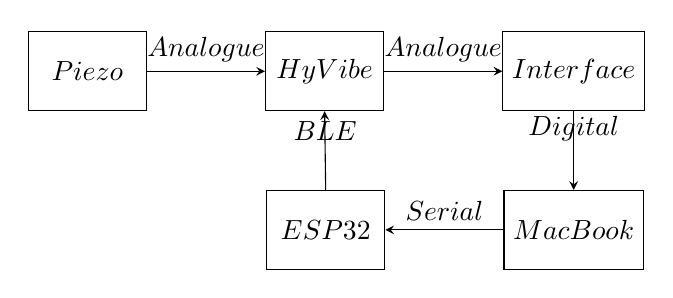
\begin{tikzpicture}
     
    \node[draw,
        minimum height=1cm,
        minimum width=1.5cm,
        fill=white]
        (piezo) at (0,0){$Piezo$};
    
    \node[draw,
        minimum height=1cm,
        minimum width=1.5cm,
        right=1.5cm of piezo,
        fill=white]
        (hyvibe) {$HyVibe$};
    
    \node[draw,
        minimum height=1cm,
        minimum width=1.5cm,
        right=1.5cm of hyvibe,
        fill=white]
        (interface) {$Interface$};
    
    \node[draw,
        minimum height=1cm,
        minimum width=1.5cm,
        below=1cm of interface,
        fill=white]
        (macbook) {$MacBook$};
    
    \node[draw,
        minimum height=1cm,
        minimum width=1.5cm,
        left=1.5cm of macbook,
        fill=white]
        (esp) {$ESP32$};
    
    \draw[-stealth] (piezo.east) -- (hyvibe.west)
        node[midway,above]{$Analogue$};
    
    \draw[-stealth] (hyvibe.east) -- (interface.west)
        node[midway,above]{$Analogue$};
    
    \draw[-stealth] (interface.south) -- (macbook.north)
        node[midway,above]{$Digital$};
    
    \draw[-stealth] (macbook.west) -- (esp.east)
        node[midway,above]{$Serial$};
    
    \draw[-stealth] (esp.north) -- (hyvibe.south)
        node[midway,above]{$BLE$};
     
    \end{tikzpicture}
    \caption{An overview of the system architecture.}
    \label{system}
    \end{figure}

\section{Results \& Discussion}

The results of the initial prototype are promising, although this represents an ideal scenario with no other noise and only three tap locations. For the offline system, this has an
average F-measure of 0.99.

The real-time system is also tested for latency in three scenarios, first when triggered by an onset tap, then from a keyboard press from Python, and finally a button press directly from the
ESP32 board. These scenarios will determine where the sources of latency occur. The latency for the fist scenario is measured by recording the audio output from the guitar and measuring the time difference between the first audio peak in the onset and the first audio peak in the metronome.
The second scenario is measured by sending a MIDI message internally to the DAW on a key press (enter) which is recorded alongside the audio output. For the third scenario the button is pressed at the same time as a note on a MIDI keyboard, which is recorded in the DAW. 
Each scenario is tested 5 times and the average latency is calculated. For the onset trigger, the total latency is a fairly substantial 1167.4ms. Comparing this with sending
the serial message directly from the Python script via a keyboard press, the latency is 1037.4ms. Finally, when the button is used, the latency is less than 1ms.
There is a serious bottleneck in the system at the serial communication layer. The onset detection itself only accounts for an average of 130ms of latency. Other methods to relay the signal
from Python may have to be considered.

The second prototype is more realistic scenario with string sounds included in the dataset instead of the strings being baffled. This now includes two control tap scenarios, both baffled and non-baffled, and the two other non control taps both baffled and non-baffled,
so a total of 6 scenarios. The F-measure remains fairly high at 0.98.

    \begin{table}[!t]
    \caption{Table to test captions and labels.}
    \centering
    \begin{tabular}{ |c|c|c| } 
     \hline
     cell1 & cell2 & cell3 \\ 
     \hline
     cell4 & cell5 & cell6 \\ 
     cell7 & cell8 & cell9 \\ 
     \hline
    \end{tabular}
    
\end{table}


With a subjective test of the online system, it seemed that percussive taps occurring at positions over the internal braces are more likely to be misclassified as control taps, hypothesised that due to the acoustic resonance here being more similar to the saddle which is also structurally attached to
the braces. The is evaluated further by creating 2 new datasets of percussive taps, one with taps occurring above the internal braces and one with taps occurring away from the internal braces. The F-measure is then calculated for each of these datasets.
Figure shows the approximate location of these braces in the guitar under test, this will vary with different guitars, but a similar principal can be applied. This hypothesis is disproven as the F-measure for the dataset over the brace is actually higher than the 
one away from the brace.

When using the weights trained on the ``Open\_String\_Balanced'' dataset and using this to predict control onsets on the LAG guitar, this performed poorly with an F-measure of 0.240. This can be improved slightly be decreasing the classification threshold from 0.5 down to 0.3, then 0.2 and finally 0.1 reaching
a maximum F-measure of 0.264. This shows that the harmonic resonance produced by taps to the equivalent locations on different guitars vary significantly.


The weights trained on the augmented dataset are evaluated further by using the ``LAG\_playing'' dataset, a realistic scenario involving a mixture of guitar playing and different taps. This again performed quite poorly with an F-measure of 0.273 at a threshold of 0.1. 

Finally, the model is trained using the ``LAG\_playing'' dataset, which is the most likely continuing steps for implementing a releasable version of the system. For this the dataset would have to be expanded across different guitars and players, and playing techniques. When using this single dataset
from one player on one guitar, an F-measure of 0.752 is achieved. 



\section{Conclusions \& Further Work}

A CNN based approach developed for detecting downbeats in music transfers well to the task of detecting percussive onsets from a hollow bodied acoustic guitar.

The latency of the overall prototype system is high which for controlling some parameters such as starting and stopping loops will be much more noticeable than turning on and off effects such as reverb. This latency however is due to a serial interface between two devices which would be 
negated in a system with inbuilt BLE capability.

Changing guitar has a large effect on the accuracy of trained models.

The realistic playing dataset would need to be expanded significantly to create one that was representative of a variety of guitar players and styles.

To determine which locations and techniques for control taps would be the most suitable for guitar players, a user study would have to take place.

\begin{thebibliography}{00}
\bibitem{b1} Schluter, J. and Bock, S. (2014) ``Improved musical onset detection with Convolutional Neural Networks'', 2014 IEEE International Conference on Acoustics, Speech and Signal Processing (ICASSP). doi: 10.1109/icassp.2014.6854953.
\bibitem{b2} Wu, C., Dittmar, C., Southall, C., Vogl, R., Widmer, G., Hockman, J., Muller, M. and Lerch, A. (2018) ``A Review of Automatic Drum Transcription'', IEEE/ACM Transactions on Audio, Speech, and Language Processing, 26(9), pp. 1457-1483. doi: 10.1109/taslp.2018.2830113.
\bibitem{b3} C. Bay, ``Glossary of Guitar Terms,'' Mel Bay Publications, 2013.
\bibitem{b4} Jack, R., Mehrabi, A., Stockman, T. and McPherson, A. (2018) ``Action-sound Latency and the Perceived Quality of Digital Musical Instruments'', Music Perception, 36(1), pp. 109-128. doi: 10.1525/mp.2018.36.1.109.
\bibitem{b5} M. A. Rohit, A. Bhattacharjee and P. Rao, ``FOUR-WAY CLASSIFICATION OF TABLA STROKES WITH MODELS ADAPTED FROM AUTOMATIC DRUM TRANSCRIPTION'', 22nd ISMIR Conference, Nov. 2021.
\bibitem{b8} N. Srivastava, G. Hinton, A. Krizhevsky, I. Sutskever and R. Salakhutdinov, ``Dropout: a simple way to prevent neural networks from overfitting,'' J. Mach. Learn. Res. 15, 1 (January 2014), 1929–1958, 2014.
\bibitem{b9} HyVibe SA, ``HyVibe System Installation Instructions'', 2021, https://www.hyvibeguitar.com/wp-content/uploads/2021/05/HyVibe-Installation-Instructions-EN.pdf.
\bibitem{b10} HyVibe SA, ``MIDI Instructions'', 2022, https://www.hyvibeguitar.com/airturn-midi-instructions/.
\bibitem{b11} C. Southall, R. Stables and J. Hockman, ``Automatic Drum Transcription for Polyphonic Recordings Using Soft Attention Mechanisms and Convolutional Neural Networks,'' ISMIR, 2017.
\bibitem{b12} Xi, Q., Bittner, R.M., Pauwels, J., Ye, X. and Bello, J.P. 2018, "Guitarset: A dataset for guitar transcription", Proceedings of the 19th International Society for Music Information Retrieval Conference, ISMIR 2018, pp. 453.
\bibitem{b13} O'Shea, K. and Nash, R. (2015) ``An introduction to convolutional neural networks.'', ArXiv, abs/1511.08458.
\bibitem{b14} Tosi, J., Taffoni, F., Santacatterina, M., Sannino, R. and Formica, D. (2017) ``Performance Evaluation of Bluetooth Low Energy: A Systematic Review'', Sensors, 17(12), p. 2898. doi: 10.3390/s17122898.
\bibitem{b15} Martelloni, A., Mcpherson, A. and Barthet, M. (2020) "Percussive Fingerstyle Guitar through the Lens of NIME: an Interview Study", New Interfaces for Musical Expression (NIME).


\end{thebibliography}
\vspace{12pt}

\end{document}
